\section{Experiment 3 : Improve Relevance Distribution}
The results from previous experiment are a strong evidence that better structured cell architecture leads to better explanation. However, there are some cases that the purposed architectures fail to distribute relevance properly.  \addfigure{\ref{fig:rel_failed_cases}} shows such cases. \todo{Here ... should not propagate relevances to .... }

\begin{figure}[h]
\centering
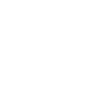
\includegraphics[draft,width=0.5\textwidth]{/sketch/placeholder}
\caption{Heatmaps of failed cases} 
\label{fig:rel_failed_cases}  %todo : figure failed cases
\end{figure}

Given the motivation above, this experiment aims to extend the proposed architectures further to better address the problem. More precisely, we consider the same classification problem as described in Section \ref{sec:exp2_prob_formulate} and propose 3 improvements, namely stationary dropout, employing gating units,  and literal connections.

\subsection{Proposal 1 :  Stationary Dropout}
Dropout is a simple regularization technique that randomly suspends activity of neurons during training. This randomized suspension allows the neurons to learn more specific representations and reduces chance of overfitting.  It is also directly related to explanation quality. \addfigure{\ref{fig:lenet_various_dropout}} shows explanations of LeNet trained with different dropout probability. 

\begin{figure}[h]
\centering
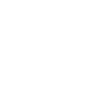
\includegraphics[draft,width=0.5\textwidth]{/sketch/placeholder}
\caption{LeNet with various dropout values} 
\label{fig:lenet_various_dropout}  
\end{figure}

However, unlike typical feedforward architectures, RNN layers are reused across time step, hence a question arises whether the same neurons in those layers should be suspended or they should be different neurons. \addfigure{\ref{fig:lstm_naive_dropout}} and \addfigure{\ref{fig:lstm_variational_dropout}} illustrates these 2 different approaches where different colors represent different dropping activities. In particular, this stationary dropout was first proposed by \cite{GalTheoreticallyGroundedApplication2016} who applied  the technique to LSTM and GRU and found improvements on language modeling tasks.

\begin{figure}
\centering
\subfloat[Naive Dropout]{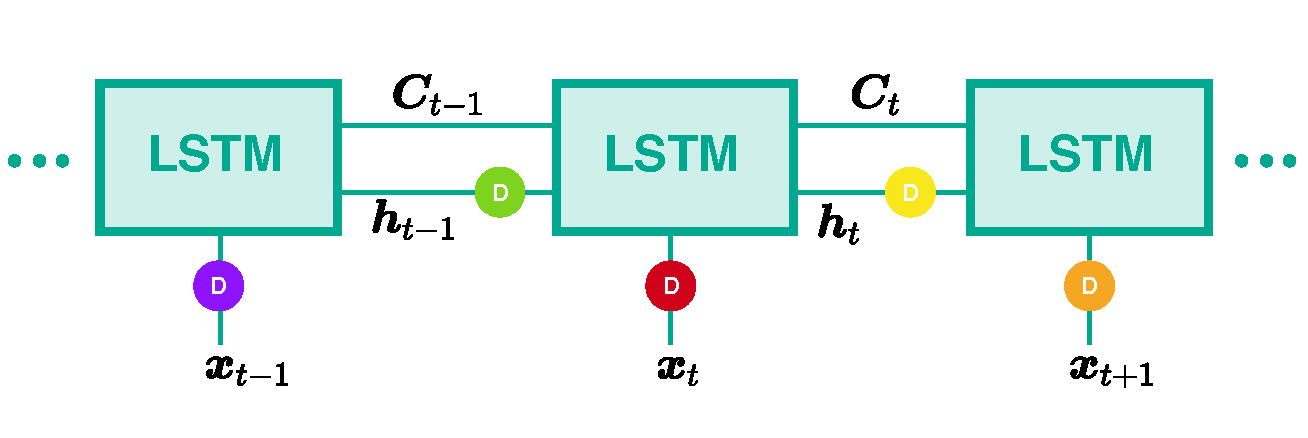
\includegraphics[width=0.8\textwidth]{sketch/lstm_naive_dropout} \label{fig:lstm_naive_dropout}} \\
\subfloat[Stationary Dropout]{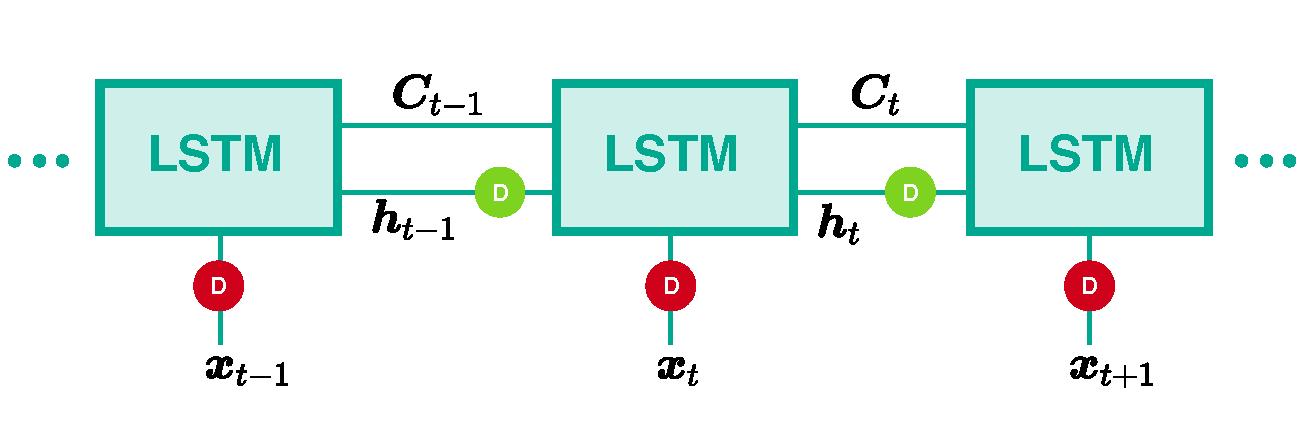
\includegraphics[width=0.8\textwidth]{sketch/lstm_variational_dropout} \label{fig:lstm_variational_dropout}}

\end{figure}

\subsection{Proposal 2 : Gating units}
\begin{figure}[h]
\centering
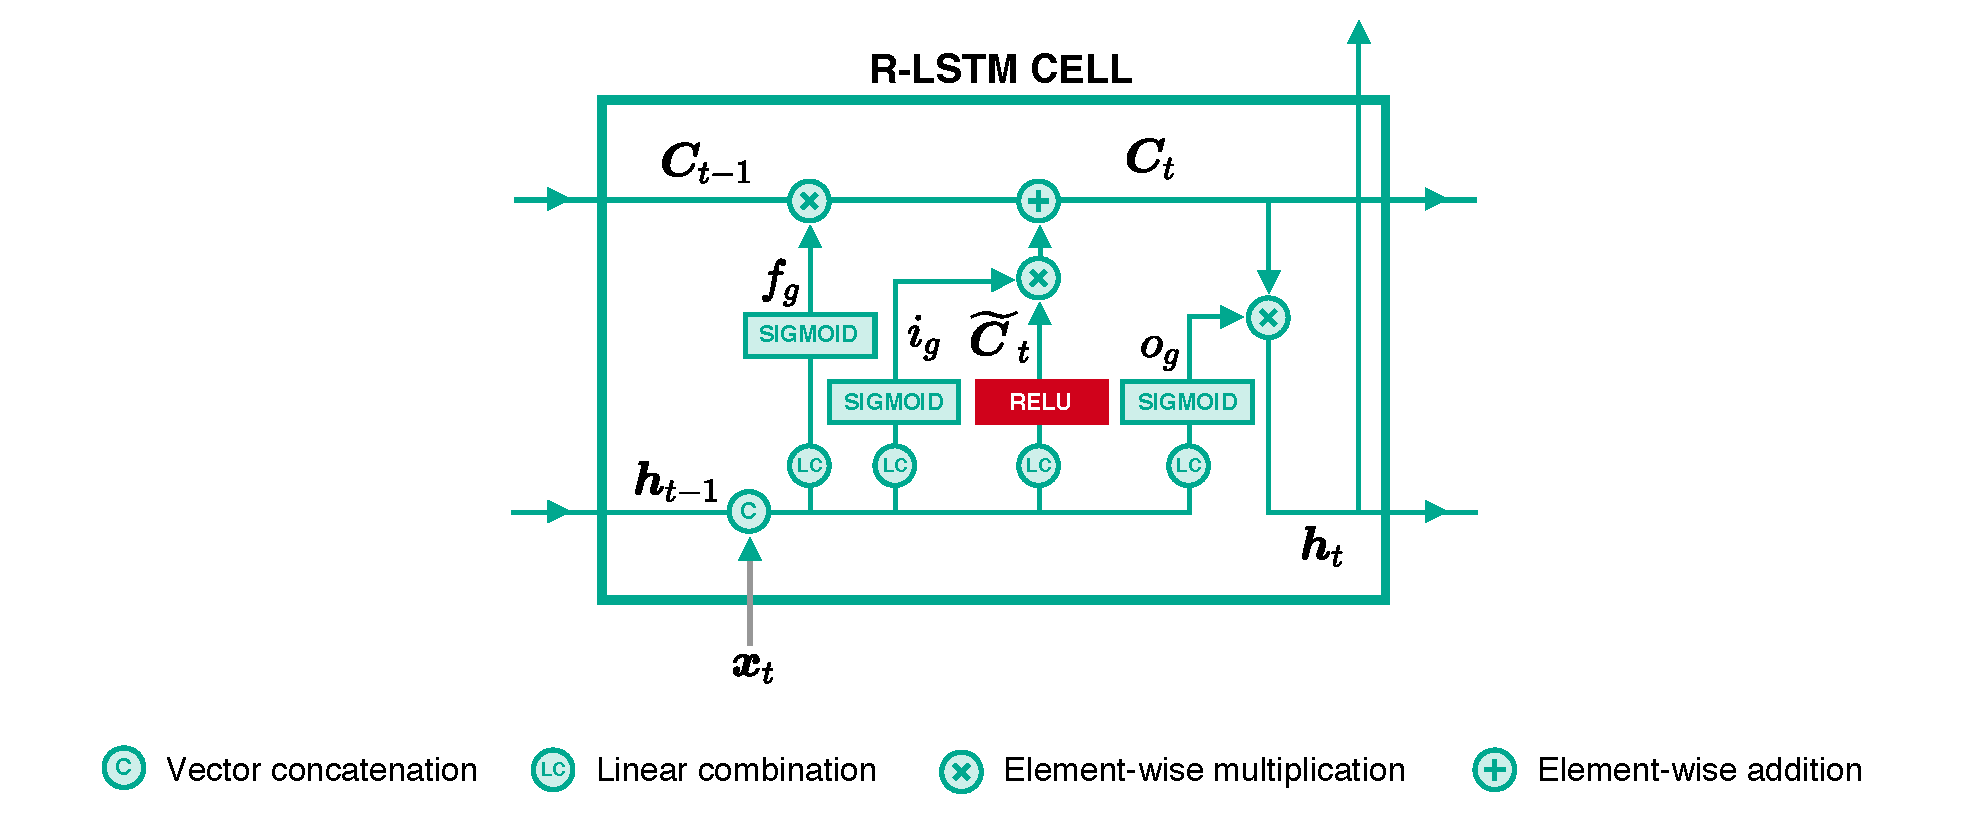
\includegraphics[width=1\textwidth]{sketch/relu_lstm}
\caption{R-LSTM Structure} 

\label{fig:relu_lstm} 
\end{figure}

It is already shown that gating units and addictive updates are critical mechanisms that enable LSTM to learn long term dependencies \cite{GreffLSTMsearchspace2017, Jozefowiczempiricalexplorationrecurrent2015a}. However, LSTM is not readily applicable for methods we are considering in this thesis. More precisely, the use of sigmoid and tanh activations violates the assumption of GB and DTD. Therefore, we propose a slight modified version of LSTM where ReLU activations are used to compute cell state candidates $\widetilde{C}_t$ instead of tanh functions. This results $C_t \in \mathbb{R}^+$, hence the tanh activation for $h_t$  is also removed.  From the following, we will refer this architecture as R-LSTM to differentiate from the original.  \addfigure{\ref{fig:relu_lstm}} presents an overview of R-LSTM architecture.


\subsection{Proposal 3 : Convolutional layer with literal connections}
As discussed in Section \ref{sec:conv}, convolution and pooling operator enable NNs to learn hierarchical representations, which are directly beneficial to explanation quality. The \rnncell{ConvDeep} architecture we proposed in Section \label{sec:rnn_cell} does not seem to exploit this properly because it has recurrent connections only layers after the convolutional and pooling layers. This can be analogically viewed that ConvDeep shares high-level features between step instead of low-level features. This might lead to obscure low-level features in the explanation. \addfigure{\ref{fig:conv_literalconn}} shows the architecture with literal connections are highlighted in red.


 \begin{figure}[h]
\centering
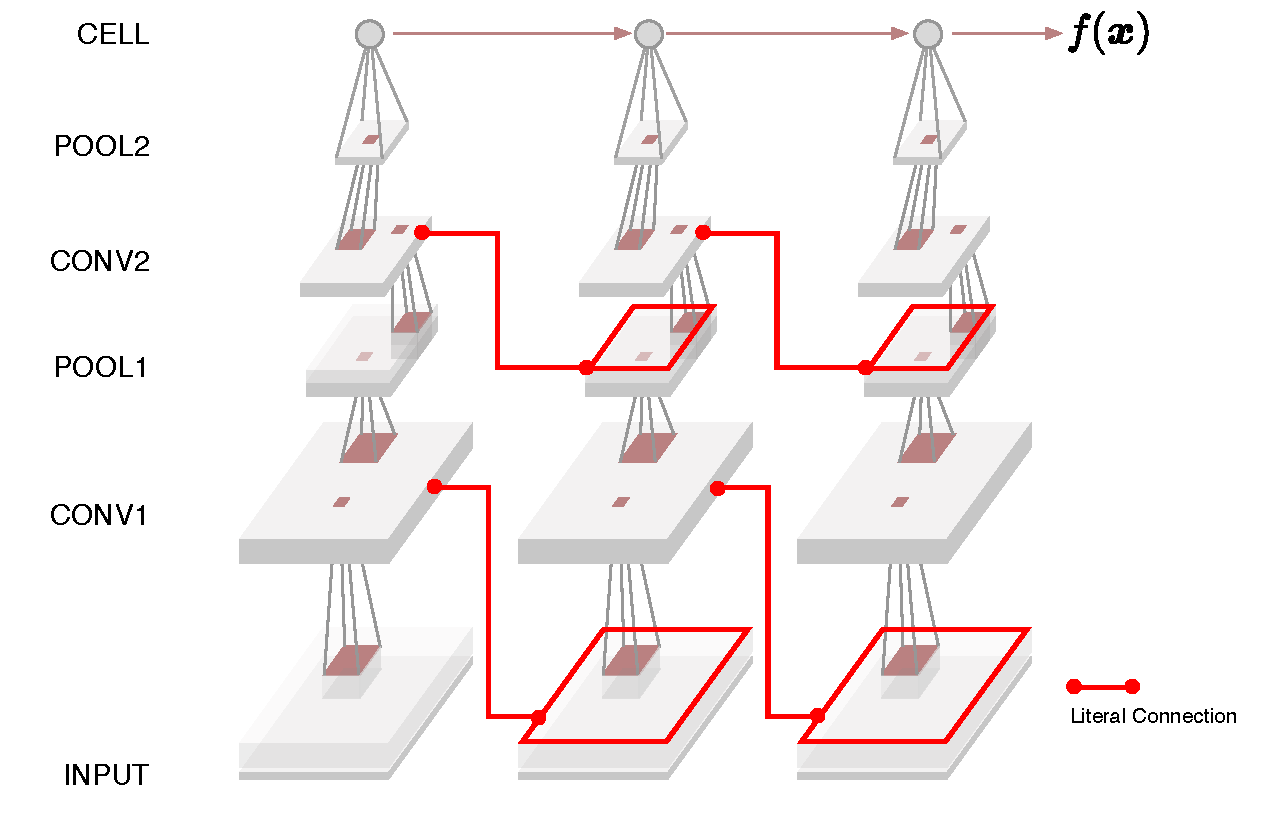
\includegraphics[width=\textwidth]{sketch/conv_literalconn}
\caption{ConvDeep with literal connections($\rnncell{ConvDeep}^+$)} 
\label{fig:conv_literalconn}
\end{figure}

Therefore, we propose an extension of ConvDeep architecture where result of convolution operator is also incorporated into the operator in the next step. We name this connection as \textit{literal connection} and refer $\rnncell{ConvDeep}^+$ to the proposed architecture. 

\subsection{Setting}
In this experiment, we divided the experiment into \todo{3?} parts. The first part focuses on stationary dropout and gating units proposal. The Deep architecture is used as the baseline. We also added one layer with 256 neurons between input and  75 R-LSTM cells to make it comparable to the Deep architecture.

The literal connection proposal is considered in the second part of the experiment where we compare the result to the \rnncell{Deep} architecture.  The last part simply combines promising improvements together.  Setting of hyperparameters are the same as in Section \ref{sec:setup}.

\subsection{Result}
Table shows accuracy and number of parameters of Deep and R-LSTM architecture. 

 \begin{figure}[h]
\centering
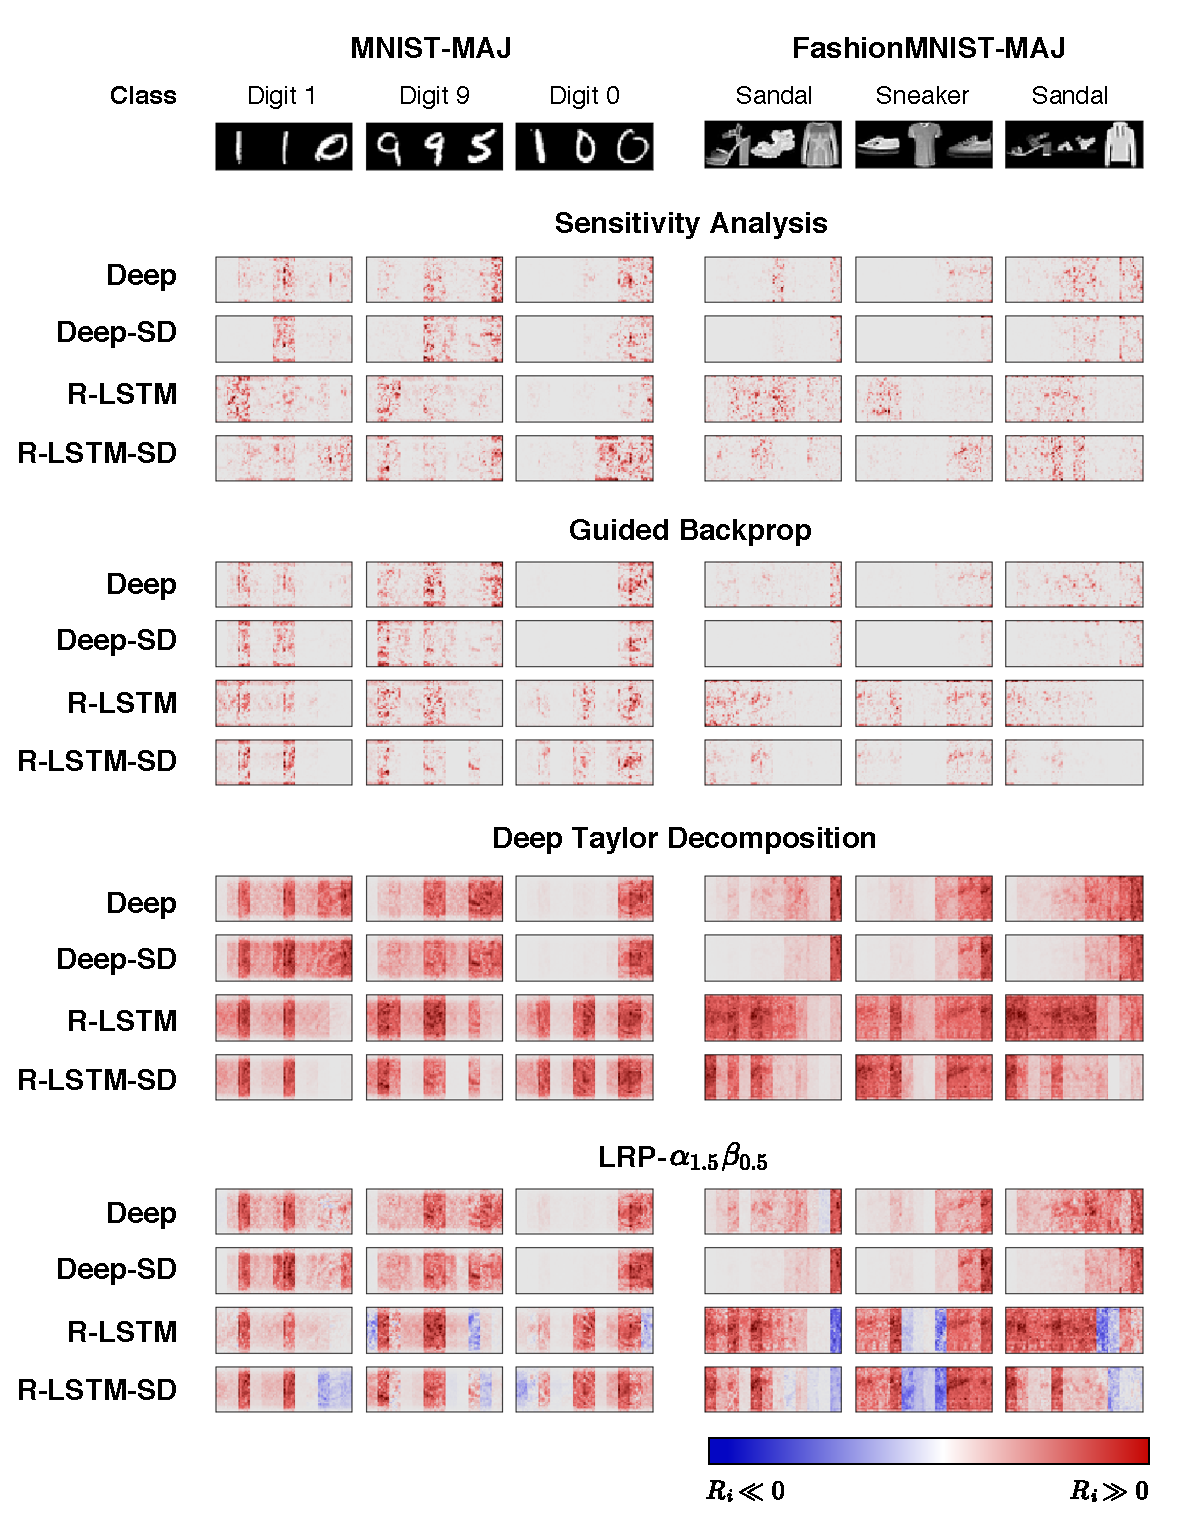
\includegraphics[width=\textwidth]{sketch/heatmap_msc_rlstm_exp}
\caption{..} 
\label{fig:heatmap_msc_rlstm_exp}
\end{figure}

 \begin{figure}[h]
\centering
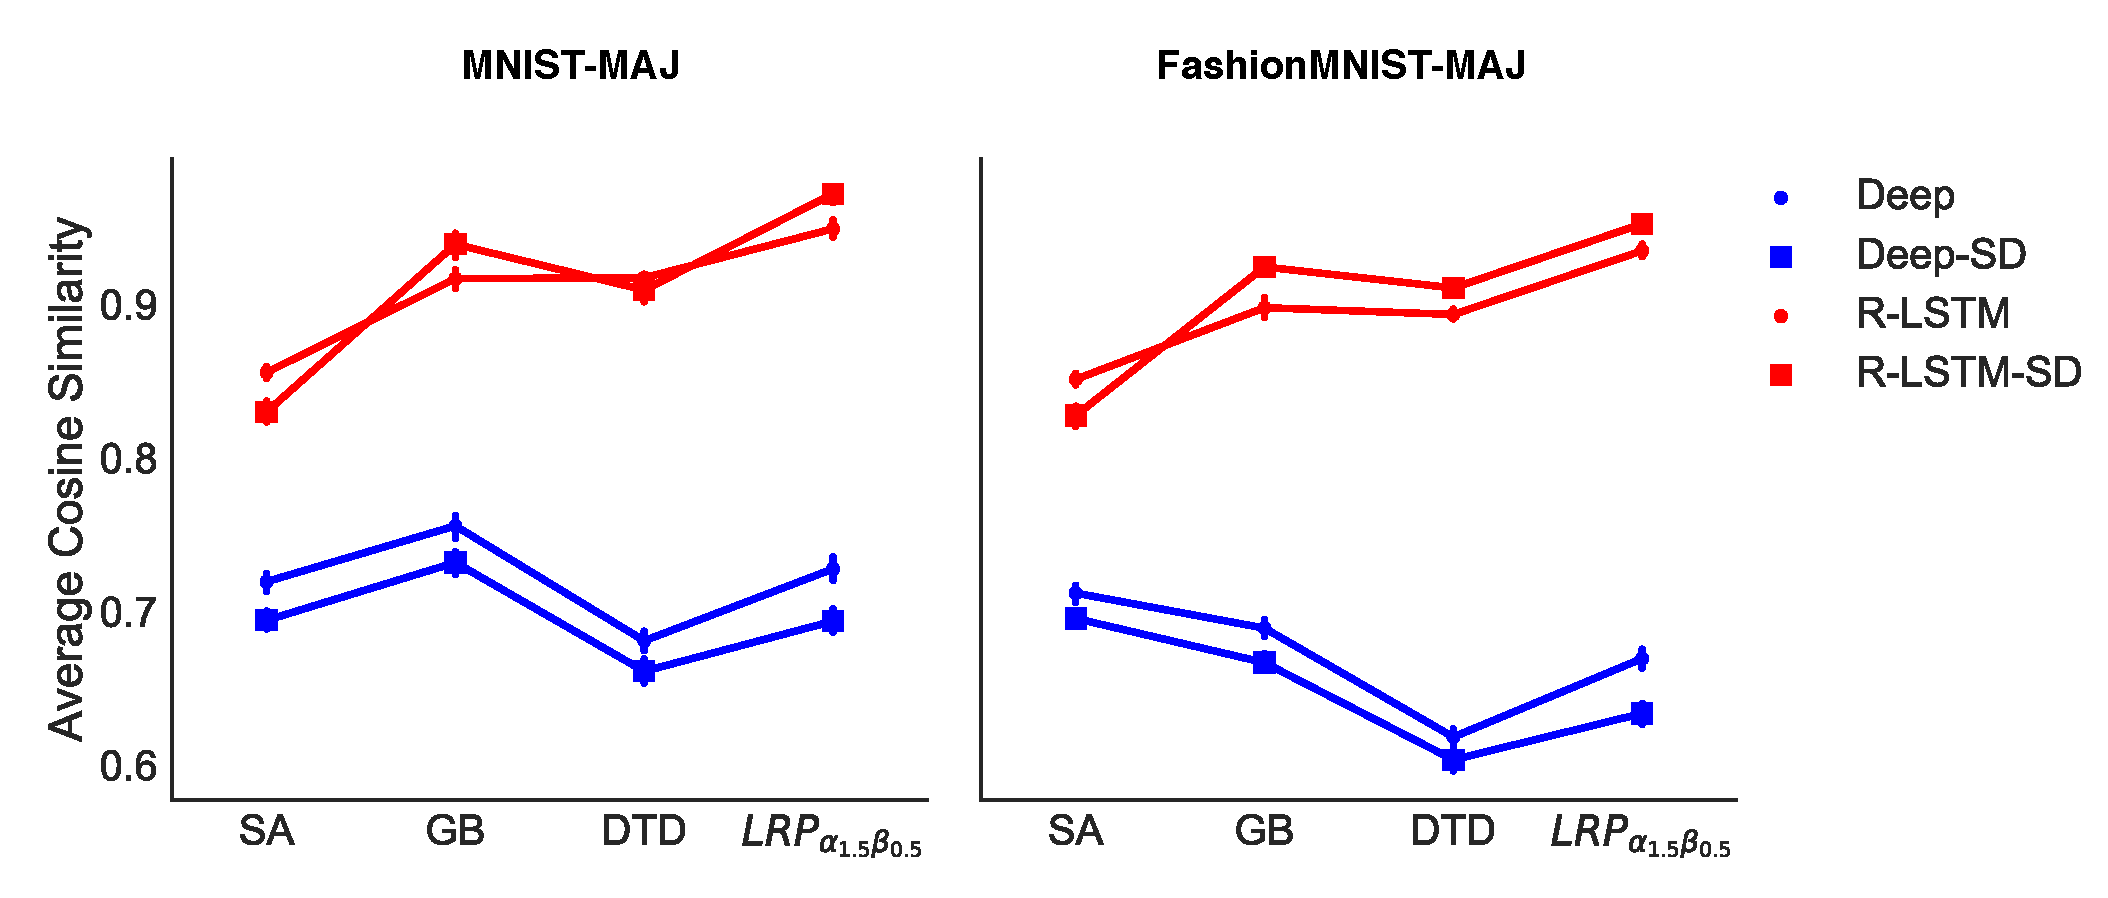
\includegraphics[width=\textwidth]{sketch/rel_dist_rlstm_exp}
\caption{..} 
\label{fig:rel_dist_rlstm_exp}
\end{figure}


ddd

\subsection{Summary}